\begin{frame}
\frametitle{LC oscillator}
\begin{columns}
  \begin{column}{0.3\textwidth}
  \begin{figure}
  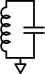
\includegraphics[scale=1.3]{LC_oscillator.pdf}
  \caption*{LC oscillator, with presumably a single mode.}
  \end{figure}
  \end{column}
  \begin{column}{0.3\textwidth}
  \begin{figure}
  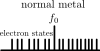
\includegraphics{normal_metal_states.pdf}
  \caption*{One oscillator mode among many electron modes}
  \end{figure}
  \end{column}
  \begin{column}{0.3\textwidth}
  \begin{figure}
  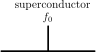
\includegraphics{superconducting_metal_states.pdf}
  \caption*{Superconducting gap: no electron modes.}
  \end{figure}
  \end{column}
\end{columns}

\pause
\begin{itemize}
  \item Superconductor below $T_c$: no electron scattering.
  \pause
  \item Low temperature: no thermal population $k_b T \ll h f_0$
  \begin{itemize}
    \item $f_0 \approx 6\,\text{GHz}$
    \item $h (1\,\text{GHz}) / k_b = 48 \, \text{mK}$. $6\, \text{GHz} \sim 288 \, \text{mK}$. Cryostat: $\sim 15\, \text{mK}$.
  \end{itemize}
\end{itemize}

\pause
A superconducting LC oscillator in a helium dilution refrigerator is literally a quantum harmonic oscillator!
\end{frame}
